\section{The Wavelet Gain Layer}

\begin{figure}[t]
  \centering
  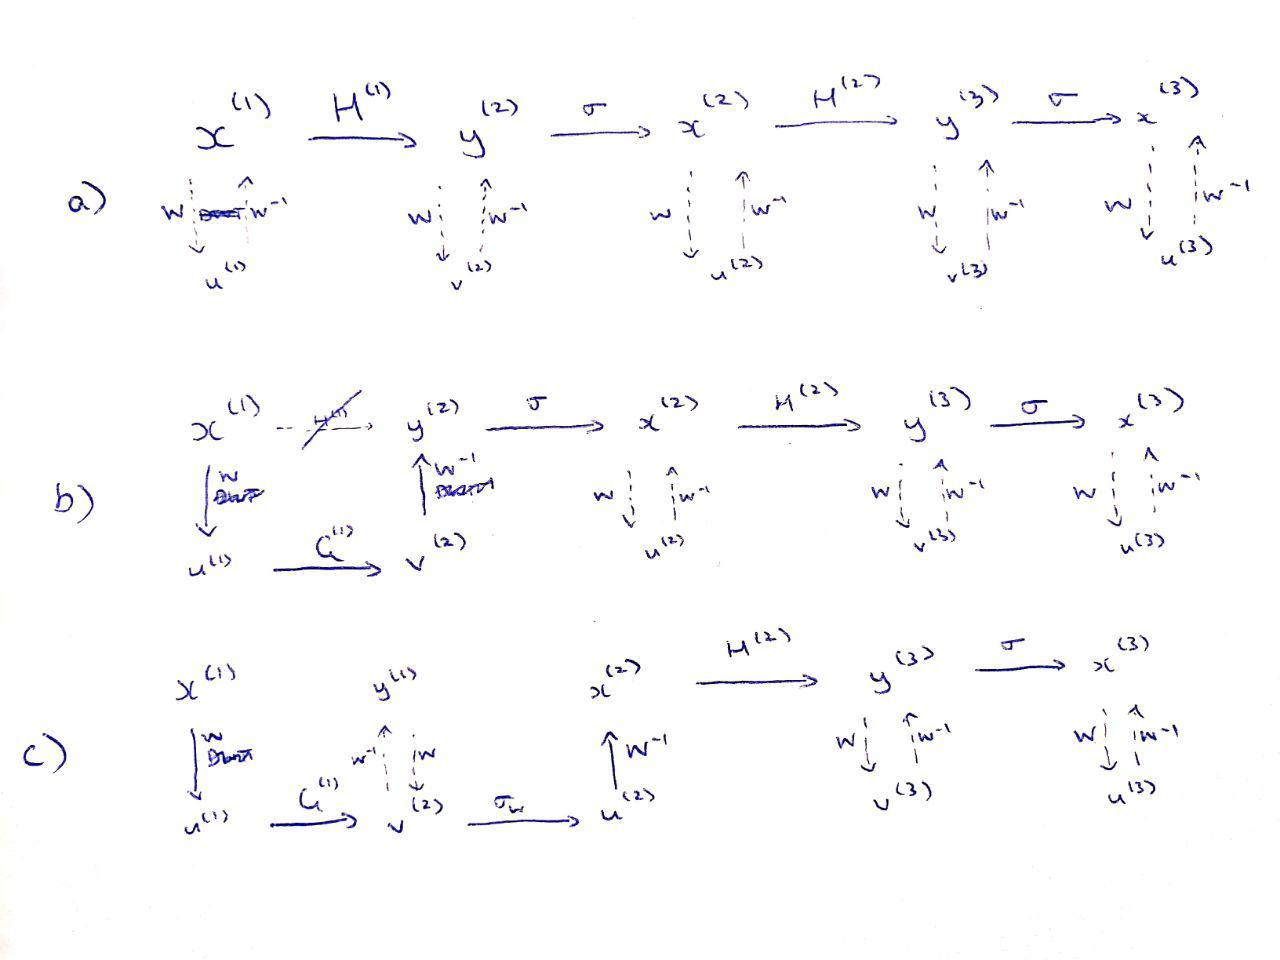
\includegraphics[width=0.8\textwidth]{\imgpath/fwd_chain.jpg}
  \mycaption{Proposed new forward pass in the wavelet domain}{Two network 
  layers with some possible options for processing. Solid lines denote the
  evaluation path and dashed lines indicate relationships. In (a) we see a
  regular convolutional neural network. We have included the dashed lines to
  make clear what we are denoting as $u$ and $v$ with respect to their
  equivalents $x$ and $y$. In (b) we get to $y^{(2)}$ through a different path.
  First we take the wavelet transform of $x^{(1)}$ to give $u^{(1)}$, apply a
  wavelet gain layer $\mathcal{G}^{(1)}$, and take the inverse wavelet transform
  to give $y^{(2)}$. The cross through $\mathcal{H}^{(1)}$ indicates that this
  path is no longer present. Note that there may not be any possible
  $\mathcal{G}^{(1)}$ to make $y^{(2)}$ from (b) equal $y^{(2)}$ from (a). In
  (c) we have stayed in the wavelet domain longer, and applied a wavelet
  nonlinearity $\sigma_w$ to give $u^{(2)}$. We then return to the pixel domain
  to give $x^{(2)}$ and continue on from there in the pixel domain.}
  \label{fig:ch6:fwd_chain}
\end{figure}


At the beginning of each stage of a neural network we have the activations
$x^{(l)}$. Naturally, all of these activations have their equivalent DWT 
coefficients $\mathtt{u}^{(l)}$ and $\DTCWT$ coefficients $u^{(l)}$. 

From \eqref{eq:ch6:conv}, convolutional layers also have intermediate
activations $y^{(l)}$. Let us differentiate these from the $x$ coefficients and
modify \eqref{eq:ch6:dwt_coeffs} and \eqref{eq:ch6:dtcwt_coeffs} to say the DWT
of $y^{(l)}$ gives $\mathtt{v}$ and the $\DTCWT$ of $y^{(l)}$ gives $v$.

We now propose the wavelet gain layers $\mathtt{G}$ and $G$ for the DWT and
$\DTCWT$ respectively, or $\mathcal{G}$ for an implementation agnostic layer.
The name `gain layer' comes from the inspiration for this chapter's work, in
that the first layer of CNN could be nearly done in the wavelet domain by
setting subband gains to 0 and 1. 

The gain layer $\mathcal{G}$ can be used instead of a convolutional layer. 
It is designed to work on the wavelet coefficients of an activation,
$\mathtt{u}$ and $u$ to give outputs $\mathtt{v}$ and $v$. 

This can be seen as breaking the convolutional path in
\autoref{fig:ch6:fwd_chain} and taking a new route to get to the next layer's
coefficients. From here, we can return to the pixel domain by taking the
corresponding inverse wavelet transform $\mathcal{W}^{-1}$. Alternatively, we
can stay in the wavelet domain and apply a wavelet based nonlinearity $\sigma_w$
to give the next layer's $u$ coefficients. Ultimately we would like to explore
architecture design with arbitrary sections in the wavelet and pixel domain, but
to do this we must first explore: 
\begin{itemize}
  \item How effective $\mathcal{G}$ is at replacing $\mathcal{H}$.
  \item How effective $\sigma_w$ is at replcaing $\sigma$.
\end{itemize}


\subsection{The DWT Gain Layer}
As mentioned previously, modifying the wavelet coefficients of a critically
sampled DWT will necessarily result in a loss of the aliasing cancelling
properties. However, in a deep neural network, this is not as obviously a bad
thing as it is for denoising or deconvolution. For this reason, we note that
there may be a problem in using a DWT, but proceed nonetheless.

For each subband in our $J$ scale system, we introduce a gain term $\mathtt{g}$. Let us specify our
input $\mathtt{u}$ has $C_l$ channels, and we would like our output $\mathtt{v}$
to have $C_{l+1}$ channels, then $\mathtt{g}$ is made up of:
\begin{align}
  \mathtt{g}_{lp} &\in \reals[C_{l+1}\x C_l\x k_{lp}\x k_{lp}] \label{eq:ch6:dwt_gstart} \\
  \mathtt{g}_{1,1} &\in \reals[C_{l+1}\x C_l\x k_{1}\x k_{1}] \\
  \mathtt{g}_{1,2} &\in \reals[C_{l+1}\x C_l\x k_{1}\x k_1] \\
      & \vdots  \nonumber \\
  \mathtt{g}_{J,3} &\in \reals[C_{l+1}\x C_l\x k_J\x k_J] \label{eq:ch6:dwt_gend}
\end{align}
%
Note that we have allowed for different kernel spatial sizes for the lowpass and for
each bandpass scale $\mathtt{g}_j$. This is to allow for the flexibility of
putting more emphasis on certain frequency areas if desired.

With these gains, we define $\mathtt{v}=\mathtt{Gu}$ to be:
\begin{align}
  \mathtt{v}_{lp}[f, \nn] &=  \sum_{c=0}^{C_l-1} \mathtt{u}_{lp}[c, \nn] \conv \mathtt{g}_{lp}[f, c, \nn] \\
  \mathtt{v}_{1,1}[f, \nn] &=  \sum_{c=0}^{C_l-1} \mathtt{u}_{1,1}[c, \nn] \conv \mathtt{g}_{1,1}[f, c, \nn] \\
  \mathtt{v}_{1,2}[f, \nn] &=  \sum_{c=0}^{C_l-1} \mathtt{u}_{1,2}[c, \nn] \conv \mathtt{g}_{1,2}[f, c, \nn] \\
                  & \vdots  \nonumber \\
  \mathtt{v}_{J,3}[f, \nn] &=  \sum_{c=0}^{C_l-1} \mathtt{u}_{J,3}[c, \nn] \conv \mathtt{g}_{J,3}[f, c, \nn] 
\end{align}
%
I.e., we do independent mixing at each of the different subbands. For $1\x 1$
kernels, this is simply a matrix multiply of the wavelet coefficients. This is shown
visually in \autoref{fig:ch6:dwt_blk_diagram}.

\subsubsection{The Output}

\begin{figure}[ht!]
  \centering
  \begin{tikzpicture}
    \matrix (m1) [minimum height=4mm, column sep=6mm, align=center]
	{
	%--------------------------------------------------------------------
		\node[coordinate]                  (m00) {};    &
		\node[coordinate]                  (m01) {};          &
		\node[dspsquare]                   (m02) {$A_0(z)$};          &
		\node[circle,draw,inner sep=1pt]   (m03) {\downsamplertext{2}}; &
    \node[dspnodeopen,dsp/label=above] (m04) {$U_{0}(z)$};          &
    \node[dspsquare]                   (m05) {$G_{0}(z)$}; &
		\node[dspnodeopen,dsp/label=above] (m06) {$V_0(z)$};          &
		\node[circle,draw,inner sep=1pt]   (m07) {\upsamplertext{2}}; &
		\node[dspsquare]                   (m08) {$S_0(z)$};          &
		\node[coordinate]                  (m09) {};          &
		\node[coordinate]                  (m0X) {};          \\
		%--------------------------------------------------------------------
		\node[dspnodefull]                 (m10) {$X(z)$};          &
		\node[coordinate]                  (m11) {};          &
		\node[coordinate]                  (m12) {};    &
		\node[coordinate]                  (m13) {};          &
		\node[coordinate]                  (m14) {};    &
		\node[coordinate]                  (m15) {};          &
		\node[coordinate]                  (m16) {};    &
		\node[coordinate]                  (m17) {};          &
		\node[coordinate]                  (m18) {};    &
		\node[dspadder]                    (m19) {};          &
		\node[]                            (m1X) {};          \\
		%--------------------------------------------------------------------
		\node[coordinate]                  (m20) {};    &
		\node[coordinate]                  (m21) {};          &
		\node[dspsquare]                   (m22) {$A_1(z)$};          &
		\node[circle,draw,inner sep=1pt]   (m23) {\downsamplertext{2}}; &
		\node[dspnodeopen,dsp/label=below] (m24) {$U_1(z)$};          &
    \node[dspsquare]                   (m25) {$G_{1}(z)$}; &
		\node[dspnodeopen,dsp/label=above] (m26) {$V_1(z)$};          &
		\node[circle,draw,inner sep=1pt]   (m27) {\upsamplertext{2}}; &
		\node[dspsquare]                   (m28) {$S_1(z)$};          &
		\node[coordinate]                  (m29) {};          &
		\node[coordinate]                  (m2X) {};          \\
		%--------------------------------------------------------------------
	};
	\draw[dspline] (m10) -- (m11);
	\draw[dspline] (m11) -- (m01);
	\draw[dspline] (m11) -- (m21);
	\foreach \i in {0,2} {
    	\draw[dspconn] (m\i1) -- (m\i2);
    	\draw[dspconn] (m\i2) -- (m\i3);
    	\draw[dspline] (m\i3) -- (m\i4);
    	\draw[dspconn] (m\i4) -- (m\i5);
    	\draw[dspline] (m\i5) -- (m\i6);
    	\draw[dspconn] (m\i6) -- (m\i7);
    	\draw[dspconn] (m\i7) -- (m\i8);
    	\draw[dspline] (m\i8) -- (m\i9);
	}
  \draw[dspconn] (m09) -- (m19);
  \draw[dspconn] (m29) -- (m19);
	\draw[dspconn] (m19) -- (m1X);
	
\end{tikzpicture}


  \mycaption{Block Diagram of 1-D DWT Gain Layer}{Here we show the low and
  highpass for a single scale 1-D DWT, Gain Layer and inverse DWT. The gain layer
  has gains $\mathtt{g}_0$ and $\mathtt{g}_1$.}
  \label{fig:ch6:dwt_gain}
\end{figure}

To explore the action of the gain layer $\mathtt{G}$ on DWT coefficients, let
use examine a 1-D, single scale, and single channel system. We want to find the
action of the layer without any nonlinearities, i.e., 
\begin{equation}
y = \mathcal{W}^{-1}\mathtt{G}\mathcal{W}x
\end{equation}
or the path taken in \autoref{fig:ch6:fwd_chain}b. 

Let us call the low and highpass analysis filters of the DWT $A_0$ and $A_1$,
and the synthesis filters $S_0$ and $S_1$ (these are normally called $H$ and
$G$, but we keep those letters reserved for the CNN and gain layer filters). 
From the perfect reconstruction property of the DWT, we know 
\begin{equation}
  A_0(z)S_0(z) + A_1(z)S_1(z) = 2
\end{equation}
and from the aliasing cancellation property of the DWT, we know:
\begin{equation}
  A_0(-z)S_0(z) + A_1(-z)S_1(z) = 0
\end{equation}
%
If we add in gains $G_0$ and $G_1$ to the low and highpass coefficients, as
shown in \autoref{fig:ch6:dwt_gain}, then the output is:
\begin{equation}
  \begin{split}
   Y(z) =& \frac{1}{2} X(z) \left[A_0(z)S_0(z)G_0(z^2) + A_1(z)S_1(z)B(z^2) \right] + \\
         & \frac{1}{2}X(-z) \left[A_0(-z)S_0(z)G_0(z^2) + A_1(-z)S_1(z)G_1(z^2) \right]
\end{split}
\end{equation}
If we let $D(z) = G_1(z^2) - G_0(z^2)$ then the above becomes:
\begin{equation}
  Y(z) = \frac{1}{2} X(z) \left[A_0(z)S_0(z)G_0(z^2) + A_1(z)S_1(z)G_1(z^2) \right] + 
         \frac{1}{2}X(-z)D(z)A_1(-z)S_1(z) \label{eq:ch6:dwt_fwd}
\end{equation}

\subsubsection{Backpropagation}\label{sec:ch6:dwt_update}
We start with the commonly known property that for a convolutional block, the
gradient with respect to the input is the gradient with respect to the output
convolved with the time reverse of the filter. More formally, if 
$Y(z) = H(z) X(z)$:
%
\begin{equation}\label{eq:ch6:backprop}
  \Delta X(z) = H(z^{-1}) \Delta Y(z)
\end{equation}
%
where $H(z^{-1})$ is the $Z$-transform of the time/space reverse of $H(z)$,
$\Delta Y(z) \triangleq \dydx{L}{Y}(z)$ is the gradient of the loss with respect
to the output, and $\Delta X(z) \triangleq \dydx{L}{X}(z)$ is the gradient of
the loss with respect to the input. 

Assume we already have access to the quantity $\Delta Y(z)$ (this is the input
to the backwards pass). \autoref{fig:ch6:bwd_pass} illustrates the
backpropagation procedure. An interesting result is that for orthogonal wavelet
transforms, $S(z^{-1}) = A(z)$, so the backwards pass of an inverse wavelet
transform is equivalent to doing a forward wavelet transform. Similarly, the
backwards pass of the forward transform is equivalent to doing the inverse
transform. The weight update gradients are then calculated by finding 
$\Delta V_i(z) = S_i(z^{-1})Y(z)$ for $i=0,\ 1$, and then convolving with the
time reverse of the saved wavelet coefficients from the forward pass -
$U_i(z^{-1})$.

\begin{equation}
  \Delta G_i(z) = \Delta V_i(z) U_i(z^{-1}) \label{eq:ch6:g_update}
\end{equation}

Unsurprisingly, the passthrough gradients have similar form to \eqref{eq:ch6:dwt_fwd}
\begin{equation}
  \Delta X(z) = \frac{1}{2} \Delta Y(z) \left[A_0(z)S_0(z)G_0(z^{-2}) + A_1(z)S_1(z)G_1(z^{-2}) \right] + 
         \frac{1}{2}\Delta Y(-z)D(z)A_1(-z)S_1(z) \label{eq:ch6:dwt_passthrough}
\end{equation}

Note that we only need to evaluate \eqref{eq:ch6:g_update},
\eqref{eq:ch6:dwt_passthrough} over the support of $G(z)$ i.e., if it is a
single number we only need to calculate $\left.\Delta G(z)\right\rvert_{z=0}$.

\begin{figure}[ht]
  \centering
  % \subfloat[]{%
    % 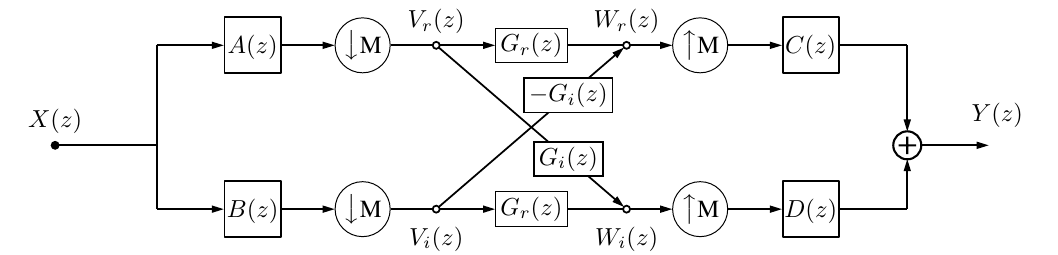
\includegraphics[width=.85\textwidth]{freqlearn/images/top_block.png}
    % \label{fig:ch6:fwd_pass}
  % }
   % \newline
  % \subfloat[]{%
    % 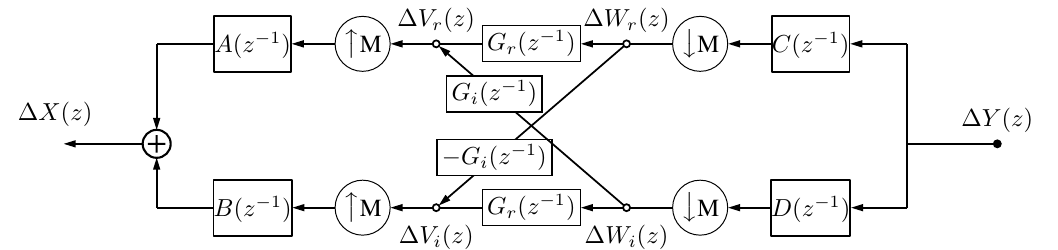
\includegraphics[width=.85\textwidth]{freqlearn/images/bottom_block.png}
    % \label{fig:ch6:bwd_pass}
  % }
  \makebox[\textwidth][c]{%
    \resizebox{1.1\textwidth}{!}{\begin{tikzpicture}
    \matrix (m1) [row sep=5mm, column sep=6mm,align=center,anchor=center]
	{
	% %--------------------------------------------------------------------
		% \node[coordinate]                  (m00) {};    &
		% \node[coordinate]                  (m01) {};          &
		% \node[dspsquare]                   (m02) {$A(z)$};          &
		% \node[circle,draw,inner sep=1pt]   (m03) {\downsamplertext{M}}; &
		% \node[dspnodeopen,dsp/label=above] (m04) {$V_r(z)$};          &
		% \node[rectangle,draw,inner sep=2pt](m05) {$G_r(z)$}; &
		% \node[dspnodeopen,dsp/label=above] (m06) {$W_r(z)$};          &
		% \node[circle,draw,inner sep=1pt]   (m07) {\upsamplertext{M}}; &
		% \node[dspsquare]                   (m08) {$C(z)$};          &
		% \node[coordinate]                  (m09) {};          &
		% \node[coordinate]                  (m0X) {};          \\
		% %--------------------------------------------------------------------
		% \node[]                            (m10) {$X(z)$};          &
		% \node[coordinate]                  (m11) {};          &
		% \node[coordinate]                  (m12) {};    &
		% \node[coordinate]                  (m13) {};          &
		% \node[coordinate]                  (m14) {};    &
		% \node[coordinate]                  (m15) {};          &
		% \node[coordinate]                  (m16) {};    &
		% \node[coordinate]                  (m17) {};          &
		% \node[coordinate]                  (m18) {};    &
		% \node[dspadder]                    (m19) {};          &
    % \node[]                            (m1X) {$Y(z)$};          \\
		% %--------------------------------------------------------------------
		% \node[coordinate]                  (m20) {};    &
		% \node[coordinate]                  (m21) {};          &
		% \node[dspsquare]                   (m22) {$B(z)$};          &
		% \node[circle,draw,inner sep=1pt]   (m23) {\downsamplertext{M}}; &
		% \node[dspnodeopen,dsp/label=below] (m24) {$V_i(z)$};          &
		% \node[rectangle,draw,inner sep=2pt](m25) {$G_r(z)$}; &
		% \node[dspnodeopen,dsp/label=below] (m26) {$W_i(z)$};          &
		% \node[circle,draw,inner sep=1pt]   (m27) {\upsamplertext{M}}; &
		% \node[dspsquare]                   (m28) {$D(z)$};          &
		% \node[coordinate]                  (m29) {};          &
		% \node[coordinate]                  (m2X) {};          \\
		% %--------------------------------------------------------------------
		% &&&&&&&&& \\
		\node[coordinate]                  (m00a) {};    &
		\node[coordinate]                  (m01a) {};          &
		\node[dspsquare]                   (m02a) {$A\left(z^{-1}\right)$};          &
		\node[circle,draw,inner sep=1pt]   (m03a) {\upsamplertext{M}}; &
		\node[dspnodeopen,dsp/label=above] (m04a) {$\Delta U_r(z)$};          &
		%\node[coordinate]                  (m05) {}; &
		\node[rectangle,draw,inner sep=2pt](m05a) {$G_r\left(z^{-1}\right)$}; &
		\node[dspnodeopen,dsp/label=above] (m06a) {$\Delta V_r(z)$};          &
		\node[circle,draw,inner sep=1pt]   (m07a) {\downsamplertext{M}}; &
		\node[dspsquare]                   (m08a) {$C\left(z^{-1}\right)$};          &
		\node[coordinate]                  (m09a) {};          &
		\node[coordinate]                  (m0Xa) {};          \\
		%--------------------------------------------------------------------
		%\node[coordinate]  (m10) {$\Delta X(z)$};          &
    \node[]                            (m10a) {$\Delta X(z)$}; &
		\node[dspadder]                    (m11a) {};          &
		\node[coordinate]                  (m12a) {};    &
		\node[coordinate]                  (m13a) {};          &
		\node[coordinate]                  (m14a) {};    &
		\node[coordinate]                  (m15a) {};          &
		\node[coordinate]                  (m16a) {};    &
		\node[coordinate]                  (m17a) {};          &
		\node[coordinate]                  (m18a) {};    &
		\node[coordinate]                  (m19a) {};          &
		\node[]                            (m1Xa) {$\Delta Y(z)$};          \\
		%--------------------------------------------------------------------
		\node[coordinate]                  (m20a) {};    &
		\node[coordinate]                  (m21a) {};          &
		\node[dspsquare]                   (m22a) {$B\left(z^{-1}\right)$};          &
		\node[circle,draw,inner sep=1pt]   (m23a) {\upsamplertext{M}}; &
		\node[dspnodeopen,dsp/label=below] (m24a) {$\Delta U_i(z)$};          &
		%\node[coordinate]                  (m25) {}; &
		\node[rectangle,draw,inner sep=2pt](m25a) {$G_r\left(z^{-1}\right)$}; &
		\node[dspnodeopen,dsp/label=below] (m26a) {$\Delta V_i(z)$};          &
		\node[circle,draw,inner sep=1pt]   (m27a) {\downsamplertext{M}}; &
		\node[dspsquare]                   (m28a) {$D\left(z^{-1}\right)$};          &
		\node[coordinate]                  (m29a) {};          &
		\node[coordinate]                  (m2Xa) {};          \\
		%--------------------------------------------------------------------
	};
	% \draw[dspline] (m10) -- (m11);
	% \draw[dspline] (m11) -- (m01);
	% \draw[dspline] (m11) -- (m21);
	% \foreach \i in {0,2} {
      % \draw[dspconn] (m\i1) -- (m\i2);
      % \draw[dspconn] (m\i2) -- (m\i3);
      % \draw[dspline] (m\i3) -- (m\i4);
      % \draw[dspconn] (m\i4) -- (m\i5);
      % \draw[dspline] (m\i5) -- (m\i6);
      % \draw[dspconn] (m\i6) -- (m\i7);
      % \draw[dspconn] (m\i7) -- (m\i8);
      % \draw[dspline] (m\i8) -- (m\i9);
	% }
	% %\draw[dspflow] (m04) --  (m06);
	% %\draw[dspflow] (m24) -- (m26);
	% \draw[dspconn] (m24) -- node[draw,pos=0.7,inner sep=2pt,fill=white] {$-G_i(z)$} (m06);
	% \draw[dspconn] (m04) -- node[draw,pos=0.7,inner sep=2pt,fill=white] {$G_i(z)$} (m26);
	% \draw[dspconn] (m09) -- (m19);
	% \draw[dspconn] (m29) -- (m19);
	% \draw[dspconn] (m19) -- (m1X);
	\draw[dspconn] (m11a) -- (m10a);
	\draw[dspconn] (m01a) -- (m11a);
	\draw[dspconn] (m21a) -- (m11a);
	\foreach \i in {0,2} {
    	\draw[dspconn] (m\i9a) -- (m\i8a);
    	\draw[dspconn] (m\i8a) -- (m\i7a);
    	\draw[dspline] (m\i7a) -- (m\i6a);
    	\draw[dspconn] (m\i6a) -- (m\i5a);
    	\draw[dspline] (m\i5a) -- (m\i4a);
    	\draw[dspconn] (m\i4a) -- (m\i3a);
    	\draw[dspconn] (m\i3a) -- (m\i2a);
    	\draw[dspline] (m\i2a) -- (m\i1a);
	}
	%\draw[dspflow] (m04) --  (m06);
	%\draw[dspflow] (m24) -- (m26);
	\draw[dspconn] (m06a) -- node[draw,pos=0.7,inner sep=2pt,fill=white] {$-G_i\left(z^{-1}\right)$} (m24a);
	\draw[dspconn] (m26a) -- node[draw,pos=0.7,inner sep=2pt,fill=white] {$G_i\left(z^{-1}\right)$} (m04a);
	\draw[dspline] (m09a) -- (m19a);
	\draw[dspline] (m29a) -- (m19a);
	\draw[dspline] (m19a) -- (m1Xa);
	
\end{tikzpicture}
}
  }
  \mycaption{Forward and backward block diagrams for $\DTCWT$ gain layer}{Based
    on Figure~4 in \cite{kingsbury_complex_2001}. Ignoring the $G$ gains, the
    top and bottom paths (through $A, C$ and $B, D$ respectively) make up the
    the real and imaginary parts for \emph{one subband} of the dual tree system.
    Combined, $A+jB$ and $C-jD$ make the complex filters necessary to have
    support on one side of the Fourier domain (see
    \autoref{fig:ch6:dtcwt_bands}). Adding in the complex gain $G_r + jG_i$, we
    can now attenuate/shape the impulse response in each of the subbands. To
    allow for learning, we need backpropagation. The bottom diagram indicates
    how to pass gradients $\Delta Y(z)$ through the layer. Note that upsampling
    has become downsampling, and convolution has become convolution with the
  time reverse of the filter (represented by $z^{-1}$ terms).}
  \label{fig:ch6:fwd_bwd}
\end{figure}



 
\subsubsection{The $\DTCWT$ Gain Layer}

The $\DTCWT$ gain layer is the same in principle to the action of the DWT gain
layer, but due to the different properties of the two transforms, the
implementation is slightly different. 
Now that we have the framework for applying a complex gain at one subband, we
can extend this to all of the subbands in the $\DTCWT$. We also reintroduce the channel
dimension. 

To do the mixing across the $C_l$ channels at each subband, giving $C_{l+1}$
output channels, we introduce the learnable filters:
%
\begin{align}
  g_{lp} &\in \reals[C_{l+1}\x C_l\x k_{lp}\x k_{lp}] \label{eq:ch6:glp} \\
  g_{1,1} &\in \complexes[C_{l+1}\x C_l\x k_1\x k_1] \\
  g_{1,2} &\in \complexes[C_{l+1}\x C_l\x k_1\x k_1] \\
      & \vdots \nonumber \\
  g_{J,6} &\in \complexes[C_{l+1}\x C_l\x k_J\x k_J]  \label{eq:ch6:gj6}
\end{align}
%
where $k, k$ are the sizes of the mixing kernels. These could be $1\x 1$ for
simple gain control, or could be larger, say $3\x 3$, to do more complex
filtering on the subbands. 

With these gains we define $v = Gu$ to be:
\begin{align}
  v_{lp}[f, \nn] &=  \sum_{c=0}^{C_l-1} u_{lp}[c, \nn] \conv g_{lp}[f, c, \nn] \\
  v_{1,1}[f, \nn] &=  \sum_{c=0}^{C_l-1} u_{1,1}[c, \nn] \conv g_{1,1}[f, c, \nn] \\
  v_{1,2}[f, \nn] &=  \sum_{c=0}^{C_l-1} u_{1,2}[c, \nn] \conv g_{1,2}[f, c, \nn] \\
                  & \vdots \nonumber \\
  v_{J,6}[f, \nn] &=  \sum_{c=0}^{C_l-1} u_{J,6}[c, \nn] \conv g_{J,6}[f, c, \nn] 
\end{align}

Note that for complex signals $a, b$ the convolution $a \conv b$ is defined as $(a_r \conv
b_r - a_i \conv b_i) + j(a_r \conv b_i + a_i \conv b_r)$. This is shown 
in Figure~\autoref{fig:ch6:dtcwt_blk_diagram}.

\subsubsection{The Output}
Unlike the DWT gain layer, the $\DTCWT$ gain layer can achieve aliasing
cancelling and therefore has a transfer function. The proof of this is done in
\autoref{app:ch6:dtcwt}. 

\begin{figure}[ht!]
  \centering
  \begin{tikzpicture}
    \matrix (m1) [row sep=5mm, column sep=6mm,align=center,anchor=center]
	{
	%--------------------------------------------------------------------
		\node[coordinate]                  (m00) {};    &
		\node[coordinate]                  (m01) {};          &
		\node[dspsquare]                   (m02) {$A_r(z)$};          &
		\node[circle,draw,inner sep=1pt]   (m03) {\downsamplertext{M}}; &
		\node[dspnodeopen,dsp/label=above] (m04) {$U_r(z)$};          &
    \node[rectangle,draw,inner sep=2pt](m05) {$G_{r}(z)$}; &
		\node[dspnodeopen,dsp/label=above] (m06) {$V_r(z)$};          &
		\node[circle,draw,inner sep=1pt]   (m07) {\upsamplertext{M}}; &
		\node[dspsquare]                   (m08) {$S_r(z)$};          &
		\node[coordinate]                  (m09) {};          &
		\node[coordinate]                  (m0X) {};          \\
		%--------------------------------------------------------------------
		\node[]                            (m10) {$X(z)$};          &
		\node[coordinate]                  (m11) {};          &
		\node[coordinate]                  (m12) {};    &
		\node[coordinate]                  (m13) {};          &
		\node[coordinate]                  (m14) {};    &
		\node[coordinate]                  (m15) {};          &
		\node[coordinate]                  (m16) {};    &
		\node[coordinate]                  (m17) {};          &
		\node[coordinate]                  (m18) {};    &
		\node[dspadder]                    (m19) {};          &
    \node[]                            (m1X) {$Y(z)$};          \\
		%--------------------------------------------------------------------
		\node[coordinate]                  (m20) {};    &
		\node[coordinate]                  (m21) {};          &
		\node[dspsquare]                   (m22) {$A_i(z)$};          &
		\node[circle,draw,inner sep=1pt]   (m23) {\downsamplertext{M}}; &
		\node[dspnodeopen,dsp/label=below] (m24) {$U_i(z)$};          &
      \node[rectangle,draw,inner sep=2pt](m25) {$G_{r}(z)$}; &
		\node[dspnodeopen,dsp/label=below] (m26) {$V_i(z)$};          &
		\node[circle,draw,inner sep=1pt]   (m27) {\upsamplertext{M}}; &
		\node[dspsquare]                   (m28) {$S_i(z)$};          &
		\node[coordinate]                  (m29) {};          &
		\node[coordinate]                  (m2X) {};          \\
		%--------------------------------------------------------------------
  };
	\draw[dspline] (m10) -- (m11);
	\draw[dspline] (m11) -- (m01);
	\draw[dspline] (m11) -- (m21);
	\foreach \i in {0,2} {
    	\draw[dspconn] (m\i1) -- (m\i2);
    	\draw[dspconn] (m\i2) -- (m\i3);
    	\draw[dspline] (m\i3) -- (m\i4);
    	\draw[dspconn] (m\i4) -- (m\i5);
    	\draw[dspline] (m\i5) -- (m\i6);
    	\draw[dspconn] (m\i6) -- (m\i7);
    	\draw[dspconn] (m\i7) -- (m\i8);
    	\draw[dspline] (m\i8) -- (m\i9);
	}
	%\draw[dspflow] (m04) --  (m06);
	%\draw[dspflow] (m24) -- (m26);
  \draw[dspconn] (m24) -- node[draw,pos=0.7,inner sep=2pt,fill=white] {$-G_{i}(z)$} (m06);
  \draw[dspconn] (m04) -- node[draw,pos=0.7,inner sep=2pt,fill=white] {$G_{i}(z)$} (m26);
  \draw[dspconn] (m09) -- (m19);
  \draw[dspconn] (m29) -- (m19);
	\draw[dspconn] (m19) -- (m1X);
	
\end{tikzpicture}


  \mycaption{Block Diagram of 1-D $\DTCWT$ Gain Layer}{Here we show the real and
  imaginary trees for a single subband. Note that while it may look similar to 
  \autoref{fig:ch6:dwt_gain}, this diagram represents the two trees for one subband rather
  than a single tree with a pair of subbands. The gain layer does a complex
  multiply, using both the real and imaginary parts of the decomposed signal.
  This preserves the shift invariance of the $\DTCWT$ for the reconstructed
  signal $Y$.
  }
  \label{fig:ch6:dtcwt_gain}
\end{figure}

For a single subband in the $\DTCWT$, the gain layer uses a complex learned
weight $g$, but otherwise produces the output $v$ in much the same way as the
DWT gain layer. \autoref{fig:ch6:dtcwt_gain} shows a single subband $\DTCWT$
based gain layer. The output of this layer is:

\begin{equation}\label{eq:ch6:dtcwt_fwd}
  Y(z) = \frac{2}{M}X(z) \left[G_r(z^{M}) \left(A_r(z)S_r(z) + A_i(z)S_i(z)\right)
  + G_i(z^{M}) \left(A_r(z)S_i(z) - A_i(z)S_r(z)\right) \right] \\
\end{equation}
See \autoref{app:ch6:dtcwt} for the derivation. The $G_r$ term modifies the
subband gain $A_rS_r + A_iS_i$ and the $G_i$ term modifies its Hilbert Pair
$A_rS_i - A_iS_r$. \autoref{fig:ch6:dtcwt_bands} show the contour plots for the
frequency support of each of these subbands. The complex gain $g$ can be used to
reshape the frequency response for each subband independently.

\subsubsection{Backpropagation}\label{sec:ch6:dtcwt_update}
If H were complex, the first term in \autoref{eq:ch6:backprop} would be
$\bar{H}(1/\bar{z})$, but as each individual block in the $\DTCWT$ is purely
real, we can use the simpler form $H(z^{-1})$. 

Again, let us calculate $\Delta V_r(z)$ and $\Delta V_i(z)$ by backpropagating
$\Delta Y(z)$ through the inverse $\DTCWT$. Again this is the same as doing the
forward $\DTCWT$ on $\Delta Y(z)$. Then the weight update equations are:

\begin{gather}
  \Delta G_r(z) = \Delta V_r(z) U_r(z^{-1}) + \Delta V_i(z) U_i(z^{-1})  \label{eq:ch6:gr_update}\\
  \Delta G_i(z) =  -\Delta V_r(z) U_i(z^{-1}) + \Delta V_i(z) U_r(z^{-1})  \label{eq:ch6:gi_update} 
\end{gather}
%
The passthrough equations have similar form to \eqref{eq:ch6:dtcwt_fwd}:
\begin{equation}\label{eq:ch6:dtcwt_passthrough}
    \Delta X(z) = \frac{2\Delta Y(z)}{M} \left[G_r(z^{-M})\left( A_r(z)S_r(z) + A_i(z)S_i(z) \right)\right. + 
      \left. jG_i(z^{-M}) \left(A_r(z)S_i(z) - A_i(z)S_r(z) \right) \right] 
\end{equation}

\begin{figure}[t]
  \centering
  \subfloat[]{%
    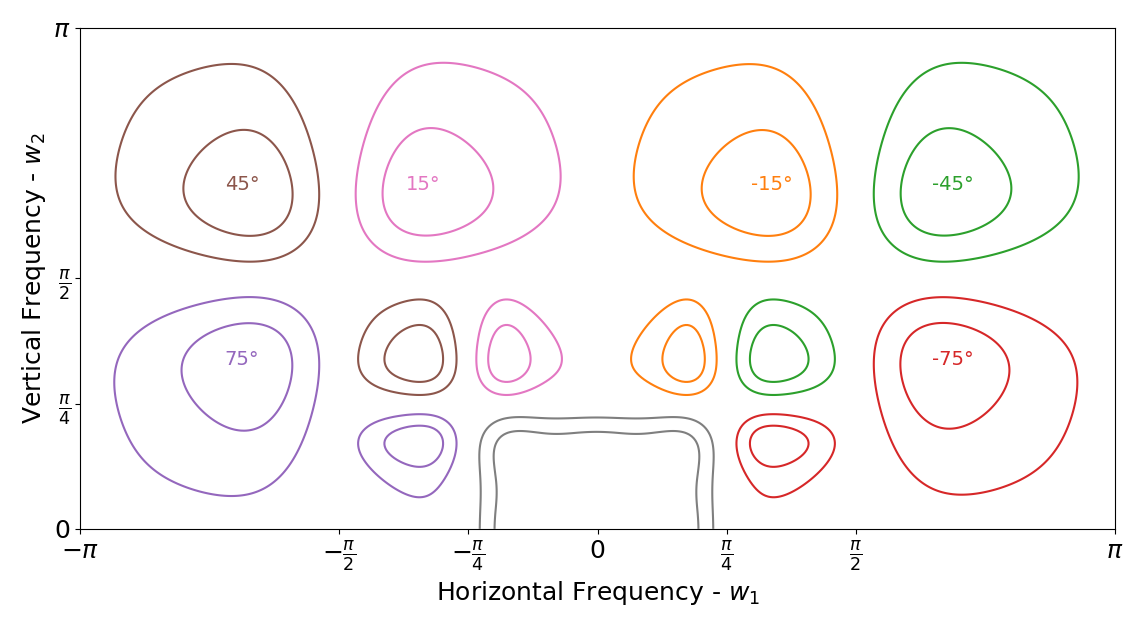
\includegraphics[height=6cm]{\imgpath/subbands.png}
    \label{fig:ch6:dtcwt_bands_freq}
  }
  \hspace{1cm}
%    \newline
  \subfloat[]{%
    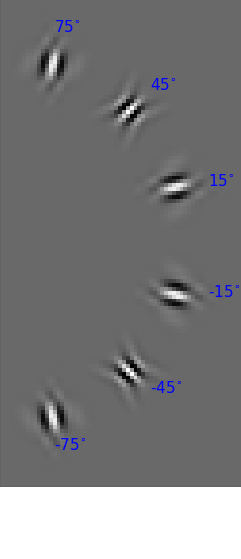
\includegraphics[height=5.7cm]{freqlearn/images/impulses.png}
    \label{fig:ch6:dtcwt_bands_impulse}
  }
  \mycaption{$\DTCWT$ subbands}{\subref{fig:ch6:dtcwt_bands_freq} -1dB and -3dB contour plots showing
  the support in the Fourier domain of the 6 subbands of the $\DTCWT$ at scales
  1 and 2, and the scale 2 lowpass. These are the product of the single side
  band filters $P(z)$ and $Q(z)$ from \autoref{thm:ch6:shiftinv}.
  \subref{fig:ch6:dtcwt_bands_impulse} The pixel domain impulse responses for
  the second scale wavelets. The Hilbert pair for each wavelet is the underlying
  sinusoid phase shifted by 90 degrees.}
  \label{fig:ch6:dtcwt_bands}
\end{figure}

\begin{figure}[t!]
  \centering
  \subfloat[]{%
    \resizebox{\textwidth}{!} {\begin{tikzpicture}[%
  path image/.style={%
    path picture={%
      \node at (path picture bounding box.center) {%
        \includegraphics[height=2.0cm]{#1}
      };
    }
  }, 
  path pic/.style={%
    path picture={%
      \node at (path picture bounding box.center) {%
        \includegraphics[height=0.8cm]{#1}
      };
    }
  }, 
  scale=0.6]

  \draw (8.8, 2.5, 5) node {\Large{$\mathtt{u}^{(l)}$}};
  \draw (10.0, 2.3, 5) node {\Large{$\conv$}};
  \draw (11.5, 2.45, 5) node {\Large{$\mathtt{g}^{(l)}$}};
  \draw (15, 2.5, 5) node {\Large{$\mathtt{v}^{(l+1)}$}};
  \draw (18.5, 2.5, 5) node {\Large{$\mathtt{u}^{(l+1)}$}};
  \draw (25, 0.8, 3.5) node {\Large{$x^{(l+1)}$}};
  \draw[<->] (10, -1.3, 2) -- (10, 0.5, 2) node[near end, right] {$C_{l+1}$};

  \draw [decorate,decoration={brace,mirror,amplitude=10pt,raise=4pt},yshift=0pt]
    (3.8,-2.5,-4) -- (4.8,-2.5,15) node [black,midway,xshift=0.8cm];
  \draw [->, fill=gray!30,ultra thick] (0.5, -2.5, 4) -- (2.5, -2.5, 4)
    node[midway, above] {$\F{DWT}$};

  \draw [decorate,decoration={brace,amplitude=10pt,raise=4pt},yshift=0pt]
    (16.5,-2.5,-4) -- (18,-2.5,15) node [black,midway,xshift=0.8cm];
  \draw [->, fill=gray!30,ultra thick] (19, -2.5, 4) -- (21.5, -2.5, 4)
    node[midway, above] {$\F{DWT}^{-1}$};
  \tikzcuboid{
  shiftx=-2.5cm,
  shifty=-2.5cm,
  shiftz=7,
  scale=0.5,
  anglex=0, 
  angley=90, 
  anglez=230,
  dimx=3, 
  dimy=3, 
  dimz=6,
  densityx=1, 
  densityy=1, 
  densityz=1,
  shade=false,
  emphedge=true,
  shadeopacity=0,
  emphstyle/.style={rounded corners=0.2pt,line width=0.3mm},
  front/.style={draw=blue!50!white,fill=blue!50!white},%
  right/.style={draw=blue!50!white,fill=blue!50!white},%
  top/.style={draw=blue!50!white,fill=blue!50!white},%
  drawxdims=true,
  dimxval=W,
  drawydims=true,
  dimyval=H,
  drawzdims=true,
  dimzval=C_l,
  }

  % Draw the 6 subband activations and their filters
  \foreach \i in {1,...,2} {
    \tikzcuboid{
    shiftx=6cm,
    shifty=-2.0cm,
    shiftz=-5+5*\i,
    scale=0.5,
    dimx=2, dimy=2, dimz=3,
    densityx=4, densityy=4, densityz=2,
    drawxdims=false,
    drawydims=false,
    dimzval=C_l,
    drawzdims=false,
    front/.style={draw=blue!50!white,fill=blue!50!white},%
    right/.style={draw=blue!50!white,fill=blue!50!white},%
    top/.style={draw=blue!50!white,fill=blue!50!white},%
    }
    \tikzcuboid{
    dimz=2,
    shiftx=12.0cm,
    }
    \tikzcuboid{
    shiftx=16.0cm,
    }
    \draw [->, fill=gray!30,ultra thick] (10+0.1*\i, -1.5, -2+2.5*\i) -- (11+0.1*\i, -1.5, -2+2.5*\i);
      % node[midway, above] {$\sigma_w$};
    \draw [->, fill=gray!30,ultra thick] (14+0.1*\i, -1.5, -2+2.5*\i) -- (15+0.1*\i, -1.5, -2+2.5*\i)
      node[midway, above] {$\sigma_w$};

    \tikzcuboid{
    shiftx=8.5cm,
    shifty=-1.0cm,
    shiftz=-5+5*\i,
    dimx=0.4, dimy=0.4, dimz=3,
    densityx=5, densityy=5, densityz=2,
    front/.style={draw=red!50!white,fill=red!50!white},%
    right/.style={draw=red!50!white,fill=red!50!white},%
    top/.style={draw=red!50!white,fill=red!50!white},%
    }
    \tikzcuboid{
    shifty=-1.5cm,
    }
    \tikzcuboid{
    shifty=-2.0cm,
    }
    \tikzcuboid{
    shifty=-2.5cm,
    }
    % \draw (8cm, -1.8cm, -15+5*\i) node {$\vdots$};
  }
  \tikzcuboid{
  shiftx=6cm,
  shifty=-2.0cm,
  shiftz=10,
  scale=0.5,
  dimx=2, dimy=2, dimz=3,
  densityx=4, densityy=4, densityz=2,
  dimxval=\frac{W}{2},
  drawxdims=true,
  dimyval=\frac{H}{2},
  drawydims=true,
  dimzval=C_l,
  drawzdims=true,
  front/.style={draw=blue!50!white,fill=blue!50!white},%
  right/.style={draw=blue!50!white,fill=blue!50!white},%
  top/.style={draw=blue!50!white,fill=blue!50!white},%
  }
  \tikzcuboid{
  shiftx=12.0cm,
  dimz=2,
  dimzval=C_{l+1},
  }
  \tikzcuboid{
  shiftx=16.0cm,
  drawxdims=false,
  drawydims=false,
  drawzdims=false
  }
  \draw [->, fill=gray!30,ultra thick] (10+3*0.1, -1.5, 5.5) -- (11+3*0.1, -1.5, 5.5);
    % node[midway, above] {$\sigma_w$};
  \draw [->, fill=gray!30,ultra thick] (14+3*0.1, -1.5, 5.5) -- (15+3*0.1, -1.5, 5.5)
      node[midway, above] {$\sigma_w$};
  \tikzcuboid{
  shiftx=8.5cm,
  shifty=-1.0cm,
  shiftz=10,
  dimx=0.4, dimy=0.4, dimz=3,
  drawxdims=false,
  drawydims=false,
  drawzdims=false,
  densityx=5, densityy=5, densityz=2,
  front/.style={draw=red!50!white,fill=red!50!white},%
  right/.style={draw=red!50!white,fill=red!50!white},%
  top/.style={draw=red!50!white,fill=red!50!white},%
  }
  \tikzcuboid{
  shifty=-1.5cm,
  }
  \tikzcuboid{
  shifty=-2.0cm,
  }
  \tikzcuboid{
  shifty=-2.5cm,
  }

  % Draw the lowpass activation and its set of filters
  \tikzcuboid{
  shiftx=6cm,
  shifty=-2.0cm,
  shiftz=30,
  scale=0.5,
  dimx=3, dimy=3, dimz=4,
  densityx=4, densityy=4, densityz=2,
  dimxval=W,
  drawxdims=true,
  dimyval=H,
  drawydims=true,
  dimzval=C_l,
  drawzdims=true,
  front/.style={draw=blue!50!white,fill=blue!50!white},%
  right/.style={draw=blue!50!white,fill=blue!50!white},%
  top/.style={draw=blue!50!white,fill=blue!50!white},%
  }
  \tikzcuboid{
  shiftx=12.0cm,
  dimz=3,
  drawxdims=false,
  drawydims=false,
  dimzval=C_{l+1},
  drawzdims=true
  }
  \tikzcuboid{
  shiftx=16.0cm,
  drawzdims=false,
  }
  \draw [->, fill=gray!30,ultra thick] (11, -1.5, 14.5) -- (12, -1.5, 14.5);
    % node[midway, above] {$\sigma_w$};
  \draw [->, fill=gray!30,ultra thick] (15, -1.5, 14.5) -- (16, -1.5, 14.5)
    node[midway, above] {$\sigma_w$};

  \tikzcuboid{
  shiftx=9cm,
  shifty=-2.75cm,
  dimx=0.8, dimy=0.8, dimz=3,
  drawxdims=false,
  drawydims=false,
  drawzdims=false,
  densityx=5, densityy=5, densityz=2,
  front/.style={draw=red!50!white,fill=red!50!white},%
  right/.style={draw=red!50!white,fill=red!50!white},%
  top/.style={draw=red!50!white,fill=red!50!white},%
  }
  \tikzcuboid{
  shifty=-2.00cm,
  }
  \tikzcuboid{
  shifty=-1.25cm,
  }
  \tikzcuboid{
  shifty=-0.5cm,
  }
  \tikzcuboid{
  shiftx=23cm,
  shifty=-2.5cm,
  shiftz=7,
  scale=0.5,
  anglex=0, 
  angley=90, 
  anglez=230,
  dimx=3, 
  dimy=3, 
  dimz=6,
  densityx=1, 
  densityy=1, 
  densityz=1,
  shade=false,
  emphedge=true,
  shadeopacity=0,
  emphstyle/.style={rounded corners=0.2pt,line width=0.3mm},
  front/.style={draw=blue!50!white,fill=blue!50!white},%
  right/.style={draw=blue!50!white,fill=blue!50!white},%
  top/.style={draw=blue!50!white,fill=blue!50!white},%
  drawxdims=true,
  dimxval=W,
  drawydims=true,
  dimyval=H,
  drawzdims=true,
  dimzval=C_{l+1},
  }
  % \draw (0, .3, 0) node {\large{$x^{(l)}$}};

\end{tikzpicture}
}
    \label{fig:ch6:dwt_blk_diagram}
  }\newline
  \vspace{1cm}
  \subfloat[]{%
    \resizebox{\textwidth}{!} {\begin{tikzpicture}[%
  path image/.style={%
    path picture={%
      \node at (path picture bounding box.center) {%
        \includegraphics[height=2.0cm]{#1}
      };
    }
  }, 
  path pic/.style={%
    path picture={%
      \node at (path picture bounding box.center) {%
        \includegraphics[height=0.8cm]{#1}
      };
    }
  }, 
  scale=0.6]
  \draw (-1, 0.8, 3.5) node {\Large{$x^{(l)}$}};
  \draw (8.5, 2.5, 0) node {\Large{$u^{(l)}$}};
  \draw (9.7, 2.3, 0) node {\Large{$\conv$}};
  \draw (11, 2.5, 0) node {\Large{$g^{(l)}$}};
  \draw (15, 2.5, 0) node {\Large{$v^{(l+1)}$}};
  \draw (18.5, 2.5, 0) node {\Large{$u^{(l+1)}$}};
  \draw (25, 0.8, 3.5) node {\Large{$x^{(l+1)}$}};
  \draw[<->] (10, -1, -2) -- (10, 0.9, -2) node[near end, right] {$C_{l+1}$};

  \draw (1.0, -2.5, -3) node {bandpass};
  \draw (2.0, -2.5, 14) node {lowpass};
  \draw [decorate,decoration={brace,mirror,amplitude=10pt,raise=4pt},yshift=0pt]
    (3.8,-2.5,-8) -- (4.8,-2.5,18) node [black,midway,xshift=0.8cm];
  \draw [->, fill=gray!30,ultra thick] (0.5, -2.5, 4) -- (2.5, -2.5, 4)
    node[midway, above] {$\DTCWT$};
  \tikzcuboid{
  shiftx=-2.5cm,
  shifty=-2.5cm,
  shiftz=7,
  scale=0.5,
  anglex=0, 
  angley=90, 
  anglez=230,
  dimx=3, 
  dimy=3, 
  dimz=6,
  densityx=1, 
  densityy=1, 
  densityz=1,
  shade=false,
  emphedge=true,
  shadeopacity=0,
  emphstyle/.style={rounded corners=0.2pt,line width=0.3mm},
  front/.style={draw=blue!50!white,fill=blue!50!white},%
  right/.style={draw=blue!50!white,fill=blue!50!white},%
  top/.style={draw=blue!50!white,fill=blue!50!white},%
  drawxdims=true,
  dimxval=W,
  drawydims=true,
  dimyval=H,
  drawzdims=true,
  dimzval=C_l,
  }

  % Draw the 6 subband activations and their filters
  \foreach \i in {1,...,5} {
    \tikzcuboid{
    shiftx=6cm,
    shifty=-2.0cm,
    shiftz=-15+5*\i,
    scale=0.5,
    dimx=2, dimy=2, dimz=3,
    densityx=4, densityy=4, densityz=2,
    drawxdims=false,
    drawydims=false,
    dimzval=C_l,
    drawzdims=false,
    front/.style={draw=blue!90!white,fill=blue!90!white},%
    right/.style={draw=blue!90!white,fill=blue!90!white},%
    top/.style={draw=blue!90!white,fill=blue!90!white},%
    }
    \tikzcuboid{
    dimz=2,
    shiftx=12.0cm,
    }
    \tikzcuboid{
    shiftx=16.0cm,
    }
    \draw [->, fill=gray!30,ultra thick] (9.8+0.08*\i, -1.5, -7+2.5*\i) -- (10.8+0.08*\i, -1.5, -7+2.5*\i);
      % node[midway, above] {$\sigma_w$};
    \draw [->, fill=gray!30,ultra thick] (13.8+0.08*\i, -1.5, -7+2.5*\i) -- (14.8+0.08*\i, -1.5, -7+2.5*\i)
      node[midway, above] {$\sigma_w$};

    \tikzcuboid{
    shiftx=8.5cm,
    shifty=-1.0cm,
    shiftz=-15+5*\i,
    dimx=0.4, dimy=0.4, dimz=3,
    densityx=5, densityy=5, densityz=2,
    front/.style={draw=red!90!white,fill=red!90!white},%
    right/.style={draw=red!90!white,fill=red!90!white},%
    top/.style={draw=red!90!white,fill=red!90!white},%
    }
    \tikzcuboid{
    shifty=-1.5cm,
    }
    \tikzcuboid{
    shifty=-2.0cm,
    }
    \tikzcuboid{
    shifty=-2.5cm,
    }
    % \draw (8cm, -1.8cm, -15+5*\i) node {$\vdots$};
  }
  \tikzcuboid{
  shiftx=6cm,
  shifty=-2.0cm,
  shiftz=15,
  scale=0.5,
  dimx=2, dimy=2, dimz=3,
  densityx=4, densityy=4, densityz=2,
  dimxval=\frac{W}{2},
  drawxdims=true,
  dimyval=\frac{H}{2},
  drawydims=true,
  dimzval=C_l,
  drawzdims=true,
  front/.style={draw=blue!90!white,fill=blue!90!white},%
  right/.style={draw=blue!90!white,fill=blue!90!white},%
  top/.style={draw=blue!90!white,fill=blue!90!white},%
  }
  \tikzcuboid{
  shiftx=12.0cm,
  dimz=2,
  dimzval=C_{l+1},
  }
  \tikzcuboid{
  shiftx=16.0cm,
  drawxdims=false,
  drawydims=false,
  drawzdims=false
  }
  \draw [->, fill=gray!30,ultra thick] (9.8+6*0.08, -1.5, 8) -- (10.8+6*0.08, -1.5, 8);
    % node[midway, above] {$\sigma_w$};
  \draw [->, fill=gray!30,ultra thick] (13.8+6*0.08, -1.5, 8) -- (14.8+6*0.08, -1.5, 8)
      node[midway, above] {$\sigma_w$};
  \tikzcuboid{
  shiftx=8.5cm,
  shifty=-1.0cm,
  shiftz=15,
  dimx=0.4, dimy=0.4, dimz=3,
  drawxdims=false,
  drawydims=false,
  drawzdims=false,
  densityx=5, densityy=5, densityz=2,
  front/.style={draw=red!90!white,fill=red!90!white},%
  right/.style={draw=red!90!white,fill=red!90!white},%
  top/.style={draw=red!90!white,fill=red!90!white},%
  }
  \tikzcuboid{
  shifty=-1.5cm,
  }
  \tikzcuboid{
  shifty=-2.0cm,
  }
  \tikzcuboid{
  shifty=-2.5cm,
  }

  % Draw the lowpass activation and its set of filters
  \tikzcuboid{
  shiftx=6cm,
  shifty=-2.0cm,
  shiftz=35,
  scale=0.5,
  dimx=3, dimy=3, dimz=4,
  densityx=4, densityy=4, densityz=2,
  dimxval=W,
  drawxdims=true,
  dimyval=H,
  drawydims=true,
  dimzval=C_l,
  drawzdims=true,
  front/.style={draw=blue!50!white,fill=blue!50!white},%
  right/.style={draw=blue!50!white,fill=blue!50!white},%
  top/.style={draw=blue!50!white,fill=blue!50!white},%
  }
  \tikzcuboid{
  shiftx=12.0cm,
  dimz=2,
  drawxdims=true,
  drawydims=true,
  dimzval=C_{l+1},
  drawzdims=true
  }
  \tikzcuboid{
  shiftx=16.0cm,
  drawxdims=false,
  drawydims=false,
  drawzdims=false,
  }
  \draw [->, fill=gray!30,ultra thick] (11.2, -1.5, 17.5) -- (12.0, -1.5, 17.5);
    % node[midway, above] {$\sigma_w$};
  \draw [->, fill=gray!30,ultra thick] (15.5, -1.5, 17.5) -- (16.5, -1.5, 17.5)
    node[midway, above] {$\sigma_w$};

  \tikzcuboid{
  shiftx=9cm,
  shifty=-2.75cm,
  dimx=0.8, dimy=0.8, dimz=3,
  drawxdims=false,
  drawydims=false,
  drawzdims=false,
  densityx=5, densityy=5, densityz=2,
  front/.style={draw=red!50!white,fill=red!50!white},%
  right/.style={draw=red!50!white,fill=red!50!white},%
  top/.style={draw=red!50!white,fill=red!50!white},%
  }
  \tikzcuboid{
  shifty=-2.00cm,
  }
  \tikzcuboid{
  shifty=-1.25cm,
  }
  \tikzcuboid{
  shifty=-0.5cm,
  }
  \tikzcuboid{
  shiftx=23cm,
  shifty=-2.5cm,
  shiftz=7,
  scale=0.5,
  anglex=0, 
  angley=90, 
  anglez=230,
  dimx=3, 
  dimy=3, 
  dimz=6,
  densityx=1, 
  densityy=1, 
  densityz=1,
  shade=false,
  emphedge=true,
  shadeopacity=0,
  emphstyle/.style={rounded corners=0.2pt,line width=0.3mm},
  front/.style={draw=blue!50!white,fill=blue!50!white},%
  right/.style={draw=blue!50!white,fill=blue!50!white},%
  top/.style={draw=blue!50!white,fill=blue!50!white},%
  drawxdims=true,
  dimxval=W,
  drawydims=true,
  dimyval=H,
  drawzdims=true,
  dimzval=C_{l+1},
  }
  % \draw (0, .3, 0) node {\large{$x^{(l)}$}};
  \draw [decorate,decoration={brace,amplitude=10pt,raise=4pt},yshift=0pt]
    (16.5,-2.5,-8) -- (18,-2.5,18) node [black,midway,xshift=0.8cm];
  \draw [->, fill=gray!30,ultra thick] (19, -2.5, 4) -- (21.5, -2.5, 4)
    node[midway, above] {$\DTCWT^{-1}$};

\end{tikzpicture}
}
    \label{fig:ch6:dtcwt_blk_diagram}
  }
  \mycaption{Block diagrams of proposed method to learn in the wavelet domain}{
  Activations are shaded blue and learned parameters red. Darker shades of
  blue and red indicate complex valued activations and weights, whereas the
  lighter shades indicate purely real values. The input $x^{(l)}\in
  \mathbb{R}^{C_l\x H\x W}$ is taken into the wavelet domain and each subband is
  mixed independently with $C_{l+1}$ sets of convolutional filters (this is what
  we call the `wavelet gain layer'. After mixing, a possible wavelet nonlinearity 
  $\sigma_w$ is applied to the subbands, before returning to the pixel domain
  with an inverse wavelet transform. \subref{fig:ch6:dwt_blk_diagram} shows 
  the system in the DWT domain. The DWT has fewer coefficients, and the gain
  layer requires fewer parameters; this is the simpler layer. 
  \subref{fig:ch6:dtcwt_blk_diagram} shows the $\DTCWT$
  based system. With 6 complex subbands and a larger lowpass, this is the more
  complex layer.}
  \label{fig:ch6:block_diagrams}
\end{figure}

\subsection{Examples}
\autoref{fig:ch6:examples} show example impulse responses of our layer for both
the DWT and $\DTCWT$ systems. The DWT outputs come from three random variables: a $1\x 1$ 
convolutional weight applied to each of the low-high, high-low and high-high
subbands. The $\DTCWT$ outputs come from twelve random variables. Again a $1\x
1$ convolutional weight, but now applied to six complex subbands. 
Our experiments have shown that the distribution of the normalized
cross-correlation between 512 of such randomly generated shapes for the DWT matches the
distribution for random vectors with roughly 2.8 degrees of freedom (c.f. 3
random variables in the layer). Similarly for the $\DTCWT$, the distribution of
the normalized cross-correlation matches the distribution for random vectors
with roughtly 11.5 degrees of freedom (c.f. 12 random variables in the layer).
This is particularly reassuring for the $\DTCWT$ as it is showing that there is
still representatitve power despite the redundancy of the transform.

\begin{figure}
  \centering
  \subfloat[]{%
  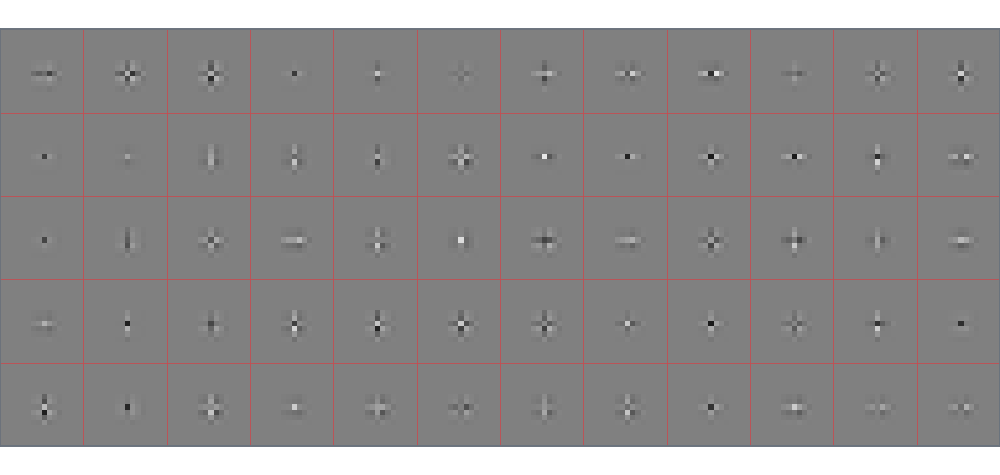
\includegraphics[width=\textwidth]{\imgpath/dwt_examples.png}
    \label{fig:ch6:dwt_examples}
  }
  \newline
  \subfloat[]{%
    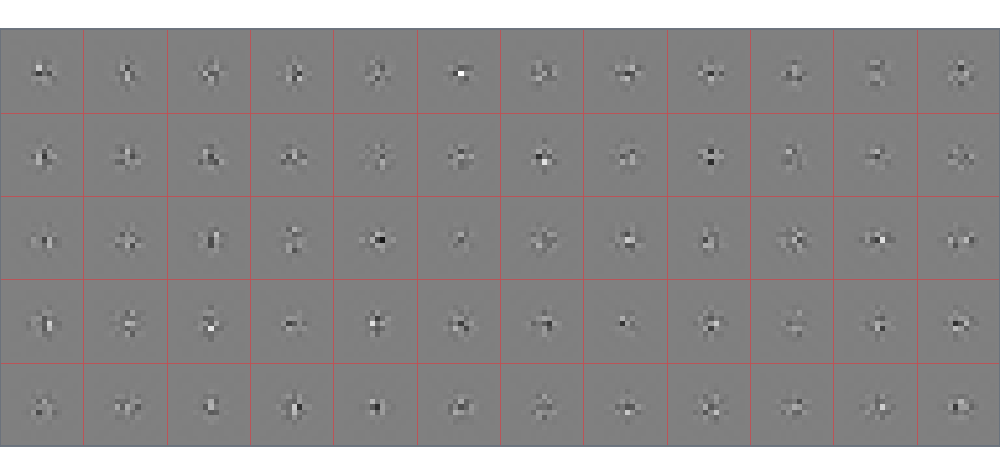
\includegraphics[width=\textwidth]{\imgpath/dtcwt_examples.png}
    \label{fig:ch6:dtcwt_examples}
  }
  \mycaption{Example outputs from an impulse input for the proposed gain layers}{
  Example outputs $y = \mathcal{W}^{-1}\mathcal{G}\mathcal{W}x$ for an impulse
  $x$ for both the DWT and $\DTCWT$ based systems. \subref{fig:ch6:dwt_examples}
  shows the outputs $y$ when $x$ is an impulse, $\mathcal{W}$ is the DWT with a
  `db2' wavelet family and $\mathcal{G} = \mathtt{G}$ is the DWT gain layer. The
  gain layer weights $\mathtt{g}_{lp}$ coefficients are set to 0 and
  $\mathtt{g}_1$ coefficients have spatial size $1\x 1$ and are sampled
  independently from a random normal of variance 1. The 60 samples come from 60
  different random initializations.
  \subref{fig:ch6:dtcwt_examples} shows the output $y$ for a $\DTCWT$ based
  system. Again, $g_{lp} = 0$ and $g_1$ has spatial size $1\x 1$. The 12 values
  in $g_1$ are independently sampled from a random normal of variance 1.}
  \label{fig:ch6:examples}
\end{figure}

